\chapter{Related Work}

\section{Reproducibility of neuroimaging pipelines across operating systems}
Neuroimaging pipelines are known to generate different results depending on the computing platform where they are compiled and executed \cite{Gla15}. Such reproducibility issues, also known as computing noise, arise from variations in harware architectures and software versions. The state-of-the-art solution to deal with these issues is to restrict studies to a single computing platform (harware and software), which has several drawbacks and, therefore, not feasible. So the best approach is to become aware of these differences.
Study conducted on FSL, Freesurfer and CIVET and different versions of GNU/Linux \cite{Gla15} shows that the differences are occuring due to the evolution of math libraries used in the operating system on which the processing takes place. A similiar study \cite{10.1371/journal.pone.0038234} concludes that the operating system updates and the software updates itself can cause diffrences in the results of neuroimaging pipelines. Results from these studies shows that there is numerical instability in these pipelines which causes reproducibility issues.\\

Explain differences.\\

\section{Potential causes of differences}
The issues regarding reproducbility could arise due to a variety of reasons other than the evolution of math libraries. The way in which the build takes place(static vs. dynamic),the nature of the language(compiler vs. interpreter), the version of the compiler used, the options used while compiling the code etc.\\ 

\section{Containers}
Computational reproducibility has become an issue of increasing importance in several research domains.	The serious challenge associated with making an experiment reproducible is the rapidly changing nature of computer enviroments. The commonly used approaches to tackle these issues are workflow softwares and virtual machines.\\

Workflow softwares provides very elegant technical solutions to the challenges of communication between diverse software tools, capturing provenance in graphically driven interfaces but most workflow systems struggle with relatively low total adoption. Virtual machines offer a more direct approach to the problem of computational reproducibility but critics highlight that it is too much of a black box approach and thus is ill-suited for reproducibility. Also it is impossible to combine multiple studies into a pipeline if each study has its own self contained virtual machine environment\cite{Boettiger:2015:IDR:2723872.2723882}.\\

A more lightweight solution is used widely among the scientific community thesedays, called containers. Container is similiar to a virtual machine, but it uses the same host operating system along with a containter manager. Container technologies has been around for a while and there are numerous implementations of it. In the year 2000,FreeBSD (4.0) featured the Jails system which focused on providing an isolated filesystem. Later came OpenSolaris, providing not only isolation services but also mechanisms related to snapshots and cloning.In 2005, OpenVZ was announced as a containerization technology supporting Linux systems. Linux containers (LXC), took advantage of the namespace concept. LXC extended the isolation property to users, processes and networking. In 2006, Google started a project which implemented a functionality to limit the resource usage. This project was later merged into the Linux kernel and it was named as "cgroups" feature. Docker, was started as an open source project in 2013, which basically added an additional layer on top of LXC, exposing additional features such as mounted storage, network port redirection, and container catalog management. Singularity , was started in 2015, with main focus on experimental reproducbility and isolation \cite{Xavier:2013:PEC:2497369.2497577}.\\ 

Containers have a closer access to operating systems than their counterpart virtualization tools such as native virtualization, paravirtualization, and hypervisors. In native virtualization, also known as full virtualization ,the guest OS is fully abstracted (completely decoupled) from the underlying hardware by the virtualization layer. Paravirtualization involves modifying the OS kernel to replace nonvirtualizable instructions with hypercalls(a hypercall is a way for the virtualized operating systems to make the hypervisor handle privileged operations) that communicate directly with the virtualization layer hypervisor \cite{citeulike:11530382}. Hypervisors present a simplified view of the native hardware to the virtual machines then they can barely access to the optimized set of instructions of actual processors.Containers subtract the hypervisor layer of the virtualization equations and relies on namespaces and cgroups in order to provide isolation and accounting of the consumed resources by the container instances.\\

\begin{center}
\begin{minipage}{0.48\linewidth}
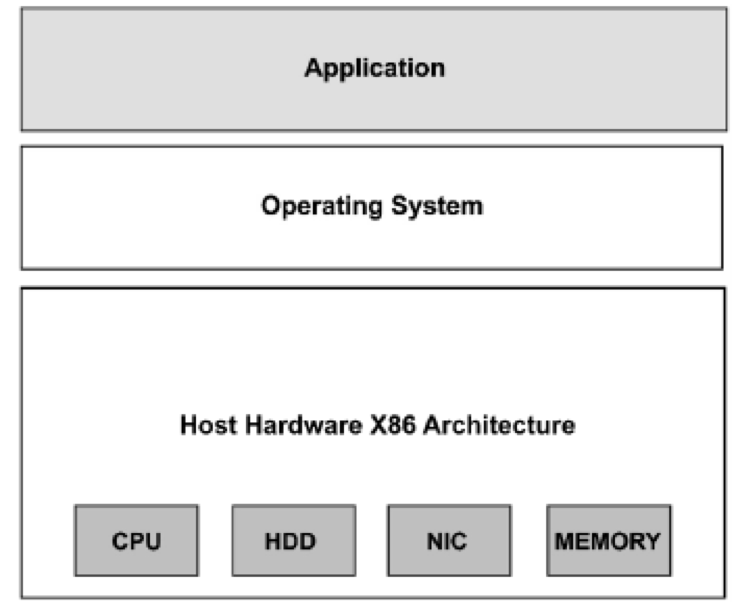
\includegraphics[height=8cm,width=\linewidth]{novirtualization.png}
\captionof{figure}{Machine with no virtualization}
\label{fig:novirtualization}
\end{minipage}%
\hfill
\begin{minipage}{0.48\linewidth}
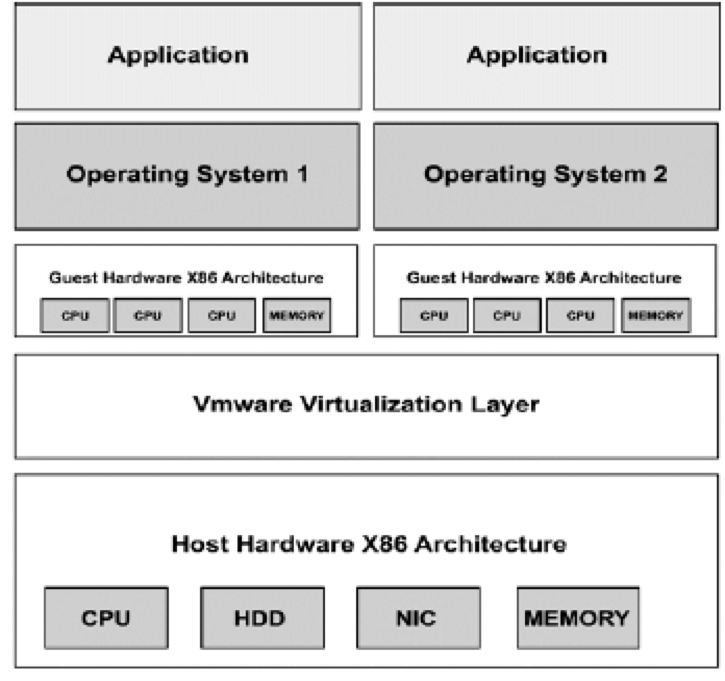
\includegraphics[height=8cm,width=\linewidth]{aftervirtualization.png}
\captionof{figure}{Machine after virtualization}
\label{fig:aftervirtualization}
\end{minipage}
\end{center}

These containers allow an user to run application and its dependancies in resource-isolated processes. Containers have a closer access to operating system services than their counterpart virtualization tools which makes their performance closer to the performance exhibited on top of native environments\cite{Xavier:2013:PEC:2497369.2497577}.\\

Even if we get access the software and tools used in an experiment, it is extremely hard to reproduce the workflow due to many undocumented assumptions, dependencies, and configurationsi \cite{7883438}. Containers can help in recreating the software environment used for the experiment in its entirety. This can help the researchers significantly since they don't have to go through the entire process of installation process. "Docker" and "Singularity" are two container based technologies widely used for containerizing the experiments.\\


What are its limitations
Include the problems listed in link https://goo.gl/zodrok\\

\subsection{Docker}
Docker provides access to virtualization facilities provided by the Linux kernel, along with some abstracted virtualized interfaces such as libvirt\footnote{\url{https://libvirt.org/}}, LXC and systemd-nspawn\footnote{\url{https://www.freedesktop.org/software/systemd/man/systemdnspawn.html}}. The control over the host's resources is provided thorugh Control Groups(cgroups) and thus it limits the amount of resources used by a container such as memory, diskspace and I/O. Docker features a layered filesystem called AuFS(Advanced Multi Layered Unification Filesystem) which allows to overlay one or more existing filesystems. This AuFS feature provides capabilites such as image versioning management and exposing base images to more specialized virtualized systems. The wide adoption of docker containers is because it can leverage the infrastructure consolidation and it exhibits a low resource footprint. Docker also boosted the adoption of service oriented architectures (e.g. microservices) because it ease the deployment of self-contained modules which are able to independantly interact with third parties using exising network protocols(e.g. web services). These service oriented architectures encourage the adoption of adaptable and extensible computational environments(e.g. workflows) \cite{Xavier:2013:PEC:2497369.2497577}. \\

The Docker software runs as a daemon on host machine. This daemon can launch containers, control their isolation level, monitor them to trigger actions, and spawn shells into running containers for administration purposes. Daemon can change iptable rules on the host and create network interfaces. The management of the images on the host machine, pushing and pulling of images from Dockerhub\footnote{\url{https://www.hub.docker.com/}}, building images from Dockerfile are all taken care by the daemon. The daemon itself runs as a root user on the host machine and it is remotely controlled through a Unix socket. Docker useas a client-server architecture.The Docker client talks to the Docker daemon and the daemon does all the heavy lifting like pushing, pulling and building images.The Docker client and daemon communicate using a REST API, over UNIX sockets or a network interface. The client and daemon need not necessarily be on the same machine\cite{docker-documentation}.\\

\begin{center}
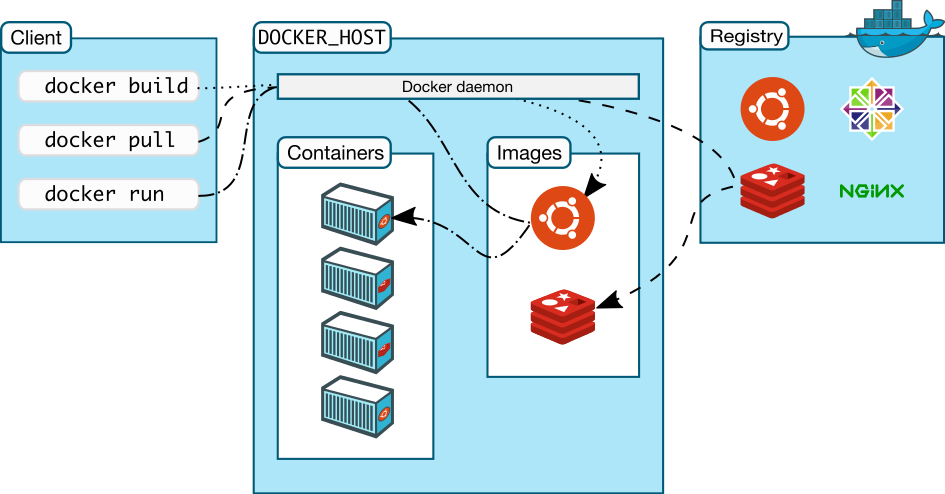
\includegraphics[width=\linewidth]{docker_architecture.png}
\captionof{figure}{Docker Architecture}
\label{fig:docker_architecture}
\end{center}

The Dockerhub is an online repository that helps developers to manage the images. Anyone who sign up on the docker hub has access to images where they can push or pull images. There is also feature for making the image creation automated with the help of git technology. Any user can create repository under his account and the repositories are namespaced using the format, "\textless developer\textgreater/\textless repository\textgreater"\cite{7742298}.\\

The wide adoption of docker containers can be attributed to both the speed and simplicity of Docker containers. The development of standardized Dockerfile format for describing and managing software containers is very straightforward. Docker helps developers to easily create standard containers for their software applications or services. For a system administrator, Docker helps in the automation of depolyment and management of business level services with the help of containers. Docker can be used as a part of virtualization layer for deploying and managing the execution environments. Another advantage is that docker containers provide reliable and predicatable execution environments and thus helps in reducing the issues related to deployment \cite{DBLP:journals/corr/MorrisVHM17}.\\

 
 
\subsection{Singularity}
Singularity is an open source initiative that harnesses the expertise of system and software engineers and researchers alike, and integrates seamlessly into common workflows for both of these groups. The primary focus of Singularity is to bring mobility of computing into both users and high performance cluster (HPC) centers alike, and integrates seamlessly into common workflows for both of these groups. Another major reason for this this open source initiative started by the Lawrence Berkeley National Laboratory (LBNL) was that, if Docker is used on HPC environments, that would mean an unreasonable level of security risk. So Docker could not be used by a large group of people that needed it greatly. Thus Singularity open source initiative came up with a product that could be used across academia and industry which is agnostic to the environment. It was developed in collaboration by HPC administrators, developers and research scientists alike. The main issue with docker running on the HPC clusters was that the daemon has to run as a root user which could lead to unnecessary risks like coercing the daemon process into granting the users escalated privileges \cite{10.1371/journal.pone.0177459}.\\

\begin{center}
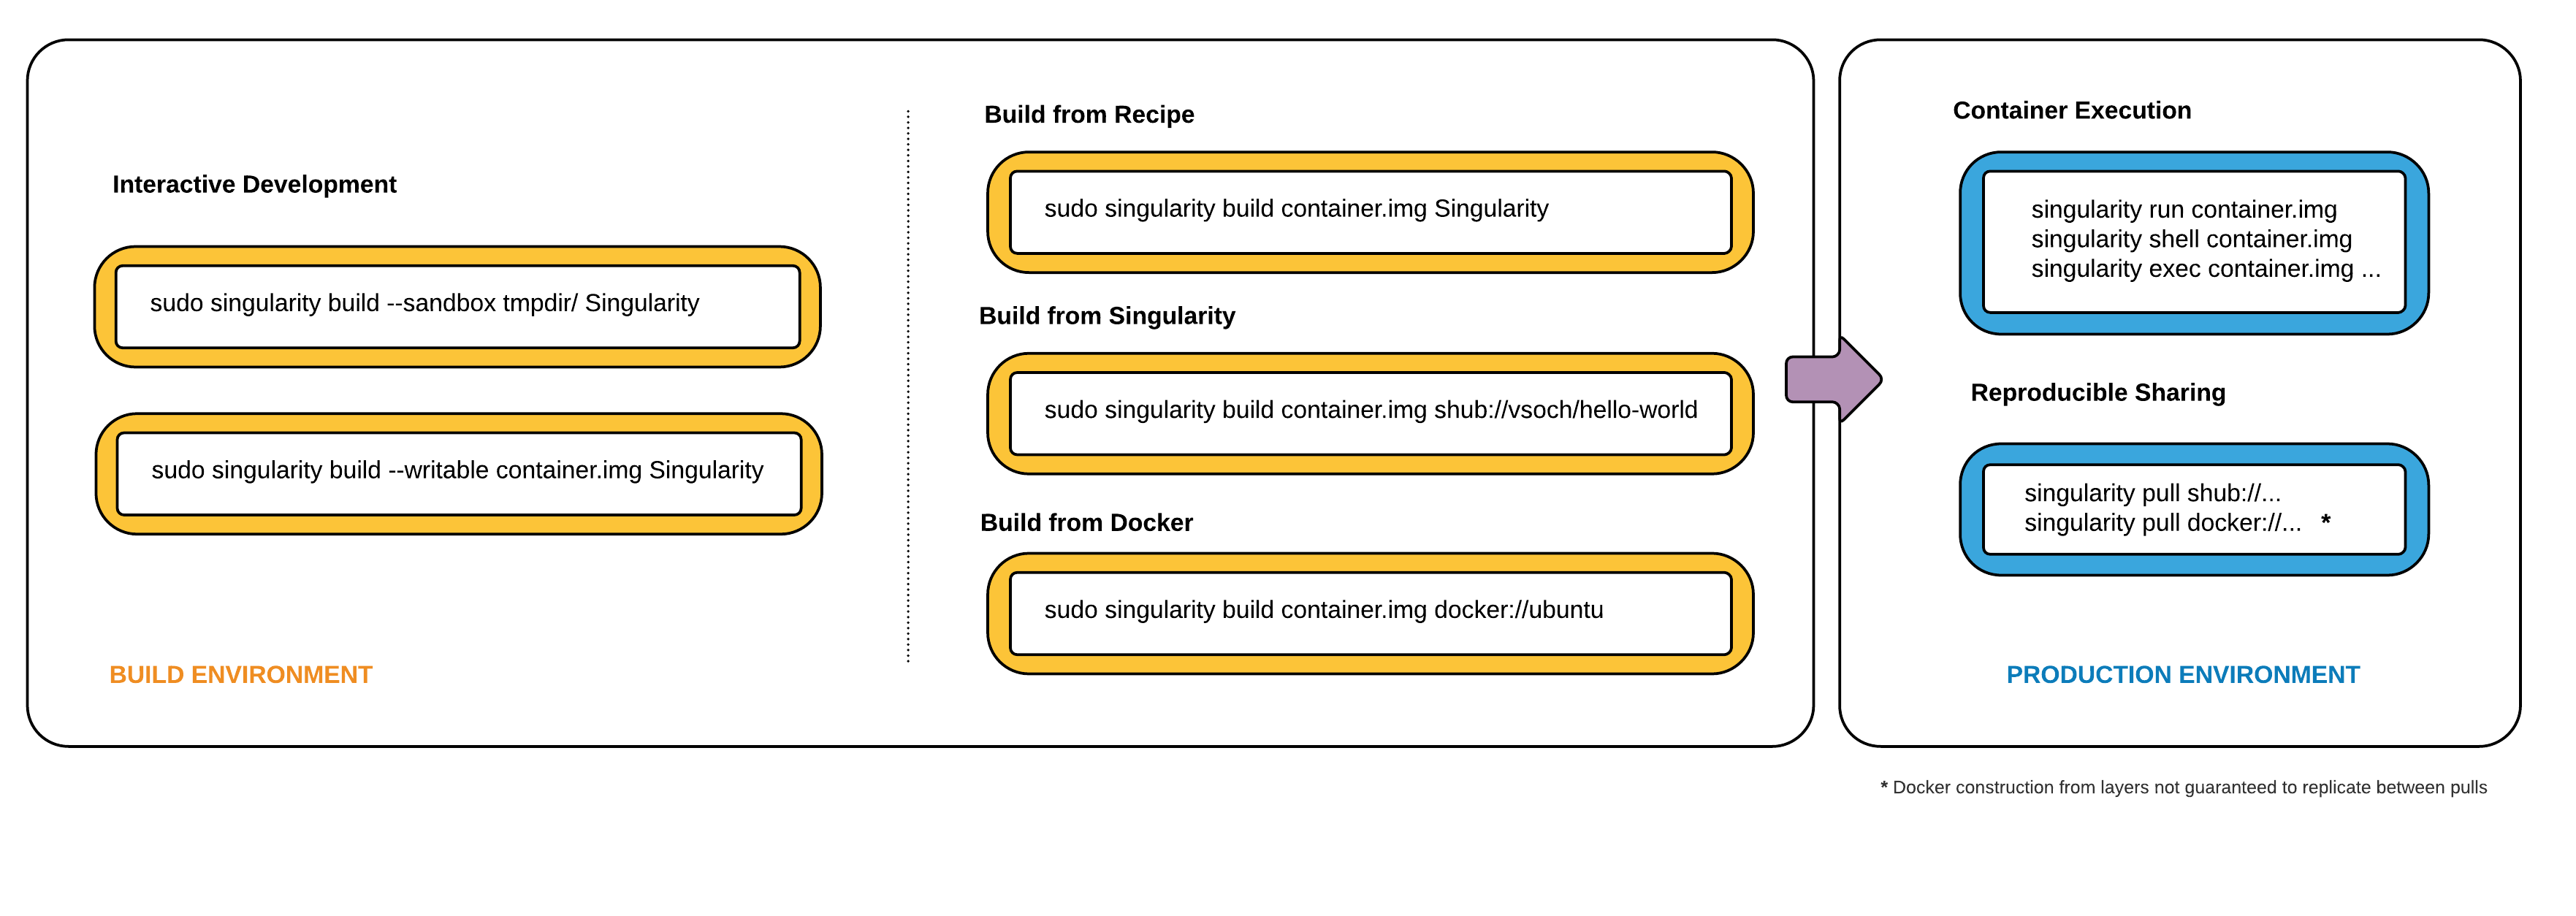
\includegraphics[width=\linewidth]{singularity.png}
\captionof{figure}{Singularity usage workflow.}
\label{fig:singularity_workflow}
\end{center}


The main goals of singularity are, 1)Mobility of compute 2)Reproducibility 3)User Freedom 4)Support on existing traditional HPC resources. The mobility of compute is the ability to create and maintian a workflow locally and being able to run the same worklfow across different hosts, operating systems or computing platforms without any problems or tweaks. Singularity achieves this by utilizing a distributable image format that encapsulates the entire container and stak into a single image file. The feature that supports reproducibility is the use of hashing. Any singularity image can make use of the hash feature to create hash and store it as metadata with built images. Users can verify these hashes to check if the image is modified or not. User freedom is granted by the ability to define their own working environment and copy the singularity image containing the entire details of that environment along with the code to a shared resource and reproduce the workflow inside that image. Singularity supports the existing and traditional HPC resources easily as installing a single package onto host operating system. Singularity is compatible with RHEL and Linux distributions dating back to Linux2.2. It natively supports the resource managers(e.g SLURM\footnote{\url{https://slurm.schedmd.com/}},Torque\footnote{\url{http://www.adaptivecomputing.com/products/open-source/torque/}}, SGE\footnote{\url{https://en.wikipedia.org/wiki/Oracle_Grid_Engine}}, etc.) and supports technologies such as InfiniBand\footnote{\url{https://en.wikipedia.org/wiki/InfiniBand}} and Lustre\footnote{\url{https://en.wikipedia.org/wiki/Lustre_(file_system)}}.\\

Singularity contiainer image encapsulates the operating system environent and all application dependencies necessary to run a defined workflow. Sinigularity container supports different kinds of uniform resource identifiers and also other container formats like Docker. http://,https://,docker://(for pulling images from docker hub),shub://(for pulling images from singularity hub), all these mechanisms are supported by singularity for obtaining the images. One another notable feature of singularity is that it does not provide a pathway for privilege escalation. At runtime, a user inside the singularity container is as same as the user as outside the container.\\
 
\subsection{Boutiques}

\section{Web platforms to run containers}
\subsection{Why do we need these platforms?}
\subsection{Examples of web computing platforms}
\subsubsection{CBRAIN}
\subsubsection{Amazon}

\section{Interposition Techniques}
\subsection{System call interception}
\subsection{Library call interception}
\subsection{Reprozip tool}
\hyperref[System Call Interception]{http://landley.net/kdocs/mirror/ols2007v1.pdf}

\section{NeuroImaging Pipelines}
The Human Connectome Project(HCP) faces the challenging task of bringing multiple magnetic resonance imaging(MRI) modalities, structural, functional, and diffusion,together into a common automated preprocessing framework across a large cohort of subjects. This framework is open and freely accessible \cite{Gla13}. The dataset from the HCP, are qualitatively different from standard neuroimaging data, having higher spatial and temporal resolutions and differing distortions. So these preprocessing pipelines creates preprocessing results that are available in standard volume and combined surface and volume spaces which makes it easier for researchers to compare the images across the neuroimaging spectrum. Since the images from the HCP dataset are cutting edge in terms of quality, it is anticipated to be widely used.

HCP minimal preprocessing pipelines are designed to minimize the amount of information actually removed from the data. These pipelines are dependant on the underlying operating system libraries for many of its functions. Hence, when there are updates in operating system versions, there could be changes in the ways which the rounding off and truncation of floating-point numbers are handled. We are trying to quantify the differences occuring due to the operating system updates on HCP preprocessing pipelines.

\begin{itemize}
 \item FSL
 \item FreeSurfer
 \item HCP Pipelines
\end{itemize}


